\documentclass[a4paper]{article}

\usepackage[fontset=fandol]{ctex}
\usepackage{amsmath, amssymb}
\usepackage{graphicx}
\usepackage[margin=2.4cm]{geometry}
\usepackage[most]{tcolorbox}
\usepackage{hyperref}
\usepackage{booktabs}
\usepackage{float}
\usepackage{enumitem}

\newtcolorbox{knowledgebox}[1]{
    enhanced, colback=blue!5!white, colframe=blue!75!black, colbacktitle=blue!75!black,
    coltitle=white, fonttitle=\bfseries, title=#1, attach boxed title to top left={yshift=-2mm, xshift=2mm},
    boxrule=1pt, sharp corners
}

\newtcolorbox{importantbox}[1]{
    enhanced, colback=yellow!10!white, colframe=yellow!80!black, colbacktitle=yellow!80!black,
    coltitle=black, fonttitle=\bfseries, title=#1, sharp corners
}

\newtcolorbox{warningbox}[1]{
    enhanced, colback=red!5!white, colframe=red!75!black, colbacktitle=red!75!black,
    coltitle=white, fonttitle=\bfseries, title=#1, sharp corners
}

\newcommand{\notetitle}{CS294/194-196 第 11 讲：LLM 时代的多智能体系统}
\newcommand{\noteauthors}{Codex 基于 Oriol Vinyals 讲座视频与官方课程页重写}
\newcommand{\notedate}{2026-04-16}
\newcommand{\videourl}{https://www.youtube.com/watch?v=ntjOxjZMaac&t=2s}
\newcommand{\videocoverpath}{../../raw/11_ntjOxjZMaac/11_ntjOxjZMaac.jpg}

\begin{document}

\begin{titlepage}
\centering
{\Large 课程讲义\par}
\vspace{1.2cm}
{\huge\bfseries \notetitle\par}
\vspace{0.8cm}
{\large \noteauthors\par}
\vspace{0.3cm}
{\large \notedate\par}
\vspace{1.2cm}
\includegraphics[width=0.82\textwidth,height=0.45\textheight,keepaspectratio]{\videocoverpath}\par
\vfill
\begin{tcolorbox}[width=0.9\textwidth, colback=black!2!white, colframe=black!60, sharp corners]
\textbf{课程}：UCB CS294/194-196 Agentic AI（Fall 2025）\par
\textbf{讲次}：Multi-Agent Systems in the Era of LLMs\par
\textbf{主讲}：Oriol Vinyals, Google DeepMind\par
\textbf{说明}：官方课程页未提供 slides，本章依据视频、字幕和课程页做 best effort 教材化重建。\par
\textbf{视频}：\href{\videourl}{\nolinkurl{\videourl}}
\end{tcolorbox}
\end{titlepage}

\tableofcontents
\newpage

\section{为什么这讲要回头讲 AlphaStar}
Oriol Vinyals 一开场就把讲座分成两部分：一部分回顾 AlphaStar 那类传统强化学习（reinforcement learning）智能体系统，一部分把这些经验重新映射到今天的 Gemini 与 LLM agents。这个组织方式非常重要，因为它说明：\textbf{多智能体系统并不是 LLM 时代凭空冒出来的新话题，而是许多老问题在新接口上的重现。}

讲者强调“ideas recirculate”。这句话的意思不是历史简单重复，而是说：很多我们今天在 LLM agent 里重新遇到的问题，例如环境定义、目标函数、工具接口、分工、协作与评估，其实早在游戏 AI 和 multi-agent reinforcement learning 里就已经被系统研究过。区别在于，今天的 environment 更开放、更模糊，用户也成了环路的一部分。

\subsection{本章小结}
这讲的起点不是“多加几个 agent 就更强”，而是把多智能体放回 agent research 的长期历史里，先搞清楚它究竟继承了哪些旧问题。

\section{什么叫 agent：从 reward maximizer 到用户驱动的复合系统}
讲者在 transcript 里非常明确地重述了一个经典定义：agent 有 goals、observations、actions，并在 environment 中循环优化 reward。这个定义来自更传统的 AI / RL 视角。在单环境、规则明确的场景里，它足够强大，也很清晰。

但讲者马上指出，今天的 agent 已经不止是“连到一个 environment 里最大化 reward”的对象。用户、聊天界面、搜索、terminal command、浏览器、外部工具和长程状态，都让 environment 本身变得更丰富，也更不封闭。于是 agent 的定义从一个简洁的 RL loop，扩展成一个用户、模型、工具与环境共同作用的复合系统。

\begin{figure}[H]
\centering
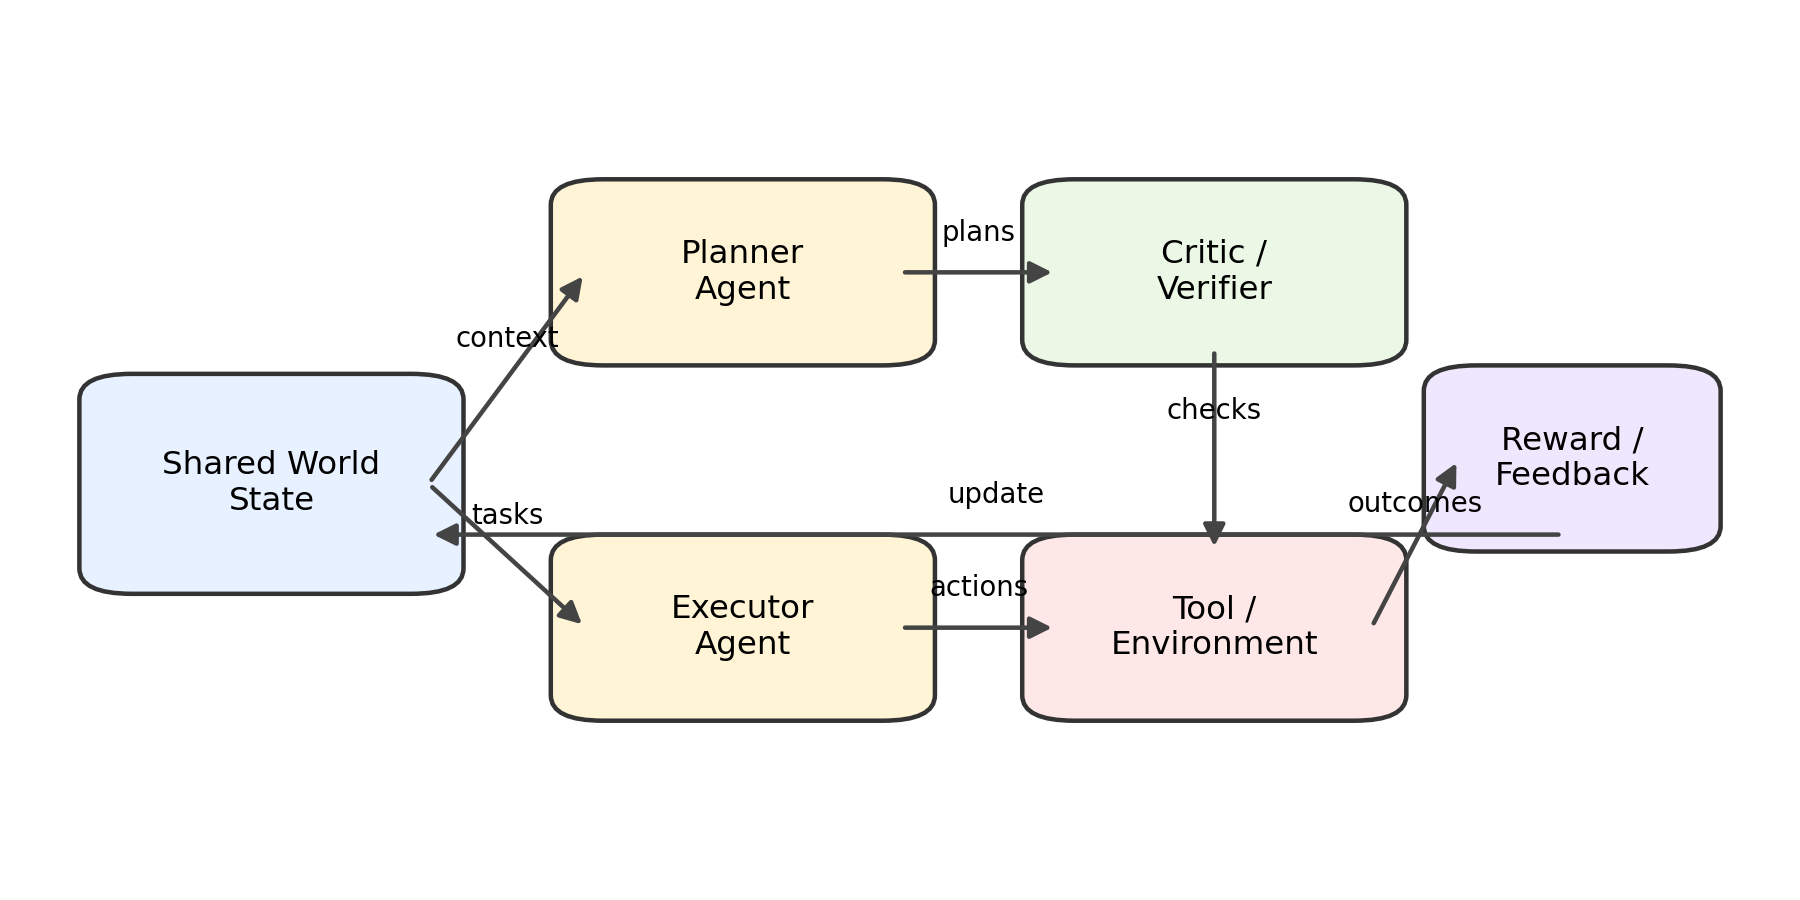
\includegraphics[width=0.88\textwidth]{figures/multi_agent_coordination.png}
\caption{从 shared world state、planner、executor、critic 到 tool/environment 的协作框架。它并不是某个特定系统的源码图，而是对本讲多智能体协调逻辑的教学化重述。}
\end{figure}

\begin{knowledgebox}{这讲对 agent 定义的关键变化}
在传统 RL 里，环境、观测、动作和奖励往往边界清晰；在 LLM 时代，用户本身也进入了环境，而 environment 又进一步扩展成搜索、终端、浏览器、API 和人类反馈共同构成的开放系统。
\end{knowledgebox}

\subsection{为什么“user 也在 loop 里”会改变一切}
一旦 agent 要服务真实用户，目标就不再只有一个显式 reward。很多时候，用户满意度、任务完成率、安全边界、策略遵守和资源消耗都要一起考虑。这让 multi-agent system 不只是 “more agents”，而是需要重新定义 coordination objective：不同子 agent 为谁工作、用什么共享状态、何时终止、何时求助用户、何时切换工具。

\subsection{本章小结}
LLM 时代的 agent 不是把传统 RL agent 套个聊天接口，而是把用户、工具和环境都纳入了同一循环，因此系统复杂度显著上升。

\section{多智能体为什么会再次重要}
如果单个 agent 已经能调用工具和规划，为什么还需要 multiple agents？这讲给出的答案，不是“因为多个 agent 更炫”，而是因为任务本身越来越复杂，很多时候自然会分解成不同角色：规划、执行、批判、验证、工具操作、环境交互。把这些功能塞进一个 monolithic policy 里不一定最稳，也不一定最可解释。

从 AlphaStar 的角度，多智能体学习（multi-agent learning）首先出现在对手、队友、协作和竞争并存的环境里。讲者提到 curriculum of difficulty、不同游戏阶段的协同，以及在复杂环境中学到的 coordination lesson。这些经验迁移到 LLM 时代后，对应的就是：是否要有 planner agent、executor agent、critic agent，是否要让不同 agent 专注不同上下文，是否要通过 self-play 或 simulated interaction 获得更强策略。

\subsection{多智能体不只是“并行”，而是结构化分工}
本讲隐含的一个重要思想是，多智能体的价值不在于多开几个线程，而在于结构化分工。不同 agent 可以拥有不同的观察窗口、工具权限、验证职责和记忆范围。这样设计的好处有三层：
\begin{itemize}[leftmargin=1.5em]
\item \textbf{降低单体复杂度}：一个 agent 不必在同一时刻既规划、又执行、又审查自己。
\item \textbf{增强可解释性}：失败时更容易定位是 planner、executor 还是 critic 的问题。
\item \textbf{更贴近组织现实}：现实工作流本来就是角色分工，而不是一个全能体包办一切。
\end{itemize}

\begin{importantbox}{多智能体的真正收益}
multi-agent 的真正收益不是“数学上 agent 数量更多”，而是把复杂任务拆成了更接近组织结构和工具权限边界的子系统。
\end{importantbox}

\subsection{本章小结}
多智能体的重要性来自任务结构，而不是技术时髦。系统之所以拆分成多个 agent，是因为开放环境里的目标、工具和责任本来就更适合分工。

\section{从游戏环境到开放 agent harness}
讲者反复回到一个对比：过去的环境是 clearly defined single environment，现在的 agent harness 则更一般，可能包含 search、terminal、browser、external APIs，甚至用户反馈本身。这一转变意味着 multi-agent systems 的难点也变了。

在游戏环境里，很多状态与奖励可以精确定义；而在开放 harness 里，状态空间更加异质，行动效果也更延迟、更难验证。比如一个 agent 可以发起搜索、读取网页、写入文件、调用终端命令，每一步都可能改变后续可见世界。此时 multi-agent coordination 不能只靠一个简单 reward signal，而需要更强的状态共享、日志记录、失败恢复和外部评测。

\subsection{为什么这和 agent engineering 直接相关}
这讲虽然来自 DeepMind 的视角，但它对今天 agent engineering 的启示非常直接：如果你希望多个 agent 协作完成任务，系统至少要有一个足够明确的共享状态表示。没有 shared state，多 agent 很容易沦为重复劳动或互相覆盖；没有明确的终止条件，多 agent 又会陷入空转和无限争论。

\begin{warningbox}{多智能体最容易被误解的地方}
如果没有共享状态、边界清晰的职责和终止机制，多智能体系统很容易比单 agent 更差。多智能体不是免费午餐，它首先是一种更复杂的系统工程。
\end{warningbox}

\subsection{本章小结}
开放 agent harness 让多智能体重新变得有价值，但同时也让 coordination 的要求更高。系统设计要解决的，不只是“谁来做”，更是“谁知道什么、谁更新什么、谁来停下”。

\section{对 LLM 时代的具体启示：哪些 old lessons 仍然成立}
讲者之所以把 AlphaStar 和 Gemini / LLM agents 放在同一讲里，不是为了做 nostalgia，而是为了提出一个判断：很多今天被重新发明的技巧，本质上早就以另一种形式出现过。最值得保留的 lessons 至少有三条。

第一，\textbf{环境抽象必须足够清晰。} 无论是游戏还是浏览器、终端、搜索 API，如果 agent 不能形成稳定的 environment model，就很难做可靠的长期规划。

第二，\textbf{coordination 需要显式结构。} 不管是 self-play、对手建模，还是 planner / executor / critic 分工，本质上都是在避免“所有行为混成一个黑箱”。

第三，\textbf{evaluation 必须贴近真实任务。} 在游戏里，胜率和奖励很明确；在 LLM agents 里，替代它们的应该是 task completion、correctness、tool-usage quality 和 user satisfaction，而不是只看表面流畅度。

\subsection{本章小结}
这讲对 LLM 时代最重要的启示，是不要把多智能体看成全新的 buzzword，而要把它看成旧的 agent ideas 在新环境里的再组织。

\section{总结与延伸}
这讲最值得带走的结论有四点。

第一，\textbf{多智能体不是 LLM 时代突然出现的新概念，它延续了长期的 agent / RL 研究传统。}

第二，\textbf{今天 agent 的 environment 比过去更开放，也更接近真实用户和真实工具，因此 coordination 问题反而更难。}

第三，\textbf{multi-agent 的价值在结构化分工，而不是 agent 数量本身。}

第四，\textbf{很多所谓“今天的新问题”，其实都可以从 AlphaStar 一类系统里找到结构前身。}

\subsection{本章小结}
Lecture 11 的真正价值，是把多智能体从时髦标签重新变回系统问题：什么是环境，什么是状态，谁来规划，谁来执行，谁来评估，以及这一切如何形成闭环。

\end{document}
